%\documentclass[aspectratio=10]{beamer} %For normal presentation (comment otherwise)
\documentclass[aspectratio=169]{beamer} %for widescreen presentation
\usetheme{Marburg}
\usefonttheme{serif}
\usepackage{ulem}
\usecolortheme{default}%albatross, crane, beetle, dove, fly, seagull, wolverine e beaver.
\setbeamertemplate{frametitle}[default][center]
%%%%%%%%%%%%%%%%%%%%%%%%%%%%%%%%%%%%%%%%%%%%%%%%%%%%%%%%%%%%%%%%%%%%%%%%%%%%%%%%%%%%%%%%%%%%%%%
%%%%%%%%%%%%%%%%%%%%%%%%%%%%%%%%%%%%%%EXTRA PACTAGES%%%%%%%%%%%%%%%%%%%%%%%%%%%%%%%%%%%%%%%%%%%
\usepackage[utf8]{inputenc}
\usepackage[T1]{fontenc}
\usepackage[scaled]{helvet}
\renewcommand*\familydefault{\sfdefault}
\usepackage[portuguese, english]{babel}
\usepackage[round]{natbib}
\usepackage{hyperref} 
\usepackage{tcolorbox}
\usepackage{graphicx} % Required for including images
\usepackage{graphics}
%\usepackage[dvips]{graphicx} 
\graphicspath{{images/}} % Location of the graphics files
\usepackage{booktabs} % Top and bottom rules for table
\usepackage[font=small,labelfont=bf]{caption}%specifies captions on tables and figures
\usepackage{amsfonts, amsmath, amsthm, amssymb} % For math fonts, symbols and environments
\usepackage{wrapfig} % Allows wrapping text around tables and figures
\usepackage{makeidx}
\usepackage{epstopdf}%adiciona imagens em formato eps no pdf.
\usepackage{subfigure}%cria ambientes de multifiguras
\usepackage{float}%coloca as figuras exatamente aonde você quer
\usepackage{times}
\usepackage{tikz}%pacote para fazer fluxogramas
\usepackage{verbatim}%
\usepackage{multicol}
\usepackage{xcolor}
\usepackage[makeroom]{cancel}
\usepackage[framemethod=tikz]{mdframed}
\usepackage{hyperref} 
\usepackage{smartdiagram}
%\smartdiagramset{uniform color list=gray!60!black for 6 items,
%back arrow disabled=false}
\usepackage{booktabs} % Top and bottom rules for table
\usepackage[font=small,labelfont=bf]{caption} % Required for specifying captions to 
\usepackage{multicol}
%%%%%%%%%%%%%%%%%%%%%%%%%%%%%%%%%%%%%%%%%%%%%%%%%%%%%%%%%%%%%%%%%%%%%%%%%%%%%%%%%%%%%%%%%%%%%
%%%%%%%%%%%%%%%%%%%%%%%%%%%%%%%%%%%%%PREAMBLE%%%%%%%%%%%%%%%%%%%%%%%%%%%%%%%%%%%%%%%%%%%%%%%%
%\subtitle{}
\author[Carreira et. al]{} 
\title{Stochastic TOC modeling for East African Rift System Lakes, a possible pre-salt analogous}
%\subtitle{Critério de seleção de amostras, Dados ANP, Bolsista IC, Estrutura PR4}
\institute{Fluminense Federal University}
\date{August 11, 2023}
%\subject{Grupo de Pesquisa em Ambientes Lacustres}
\setbeamertemplate{footline}[frame number]
%\setbeamercovered{transparent}
\setbeamertemplate{navigation symbols}{}
% Tela cheia
\hypersetup{pdfpagemode=FullScreen}
\usepackage{ragged2e}
%\justifying
%\addtobeamertemplate{headline}{} 

%%%%%%%%%%%%%%%%%%%%%%%%%%%%%PRESENTATION%%%%%%%%%%%%%%%%%%%%%%%%%%%%%%%%%%%%%%
\begin{document}
\bgroup
\makeatletter
\setbeamertemplate{footline}
\makeatother
\egroup
\scriptsize 
\addtobeamertemplate{navigation symbols}{}{\hskip6pt\raisebox{2pt}{\color{blue}\insertframenumber}}
\setcounter{framenumber}{0}



{
\usebackgroundtemplate{
\centering
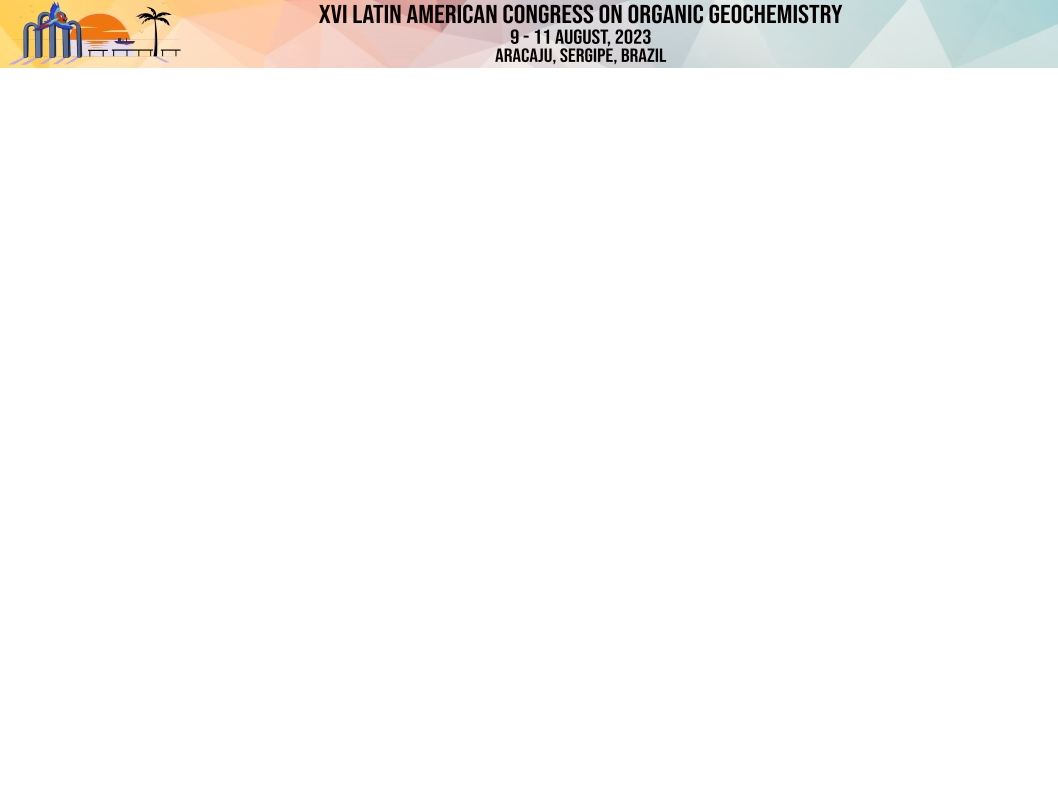
\includegraphics[width=\paperwidth,height=\paperheight]{images/fundo.jpg}
}
\begin{frame}
\maketitle
	
\end{frame}
}


%%% MOSTRAR OS OBJETIVOS DO TRABALHO
\section{Objectives}

{
\usebackgroundtemplate{
\centering
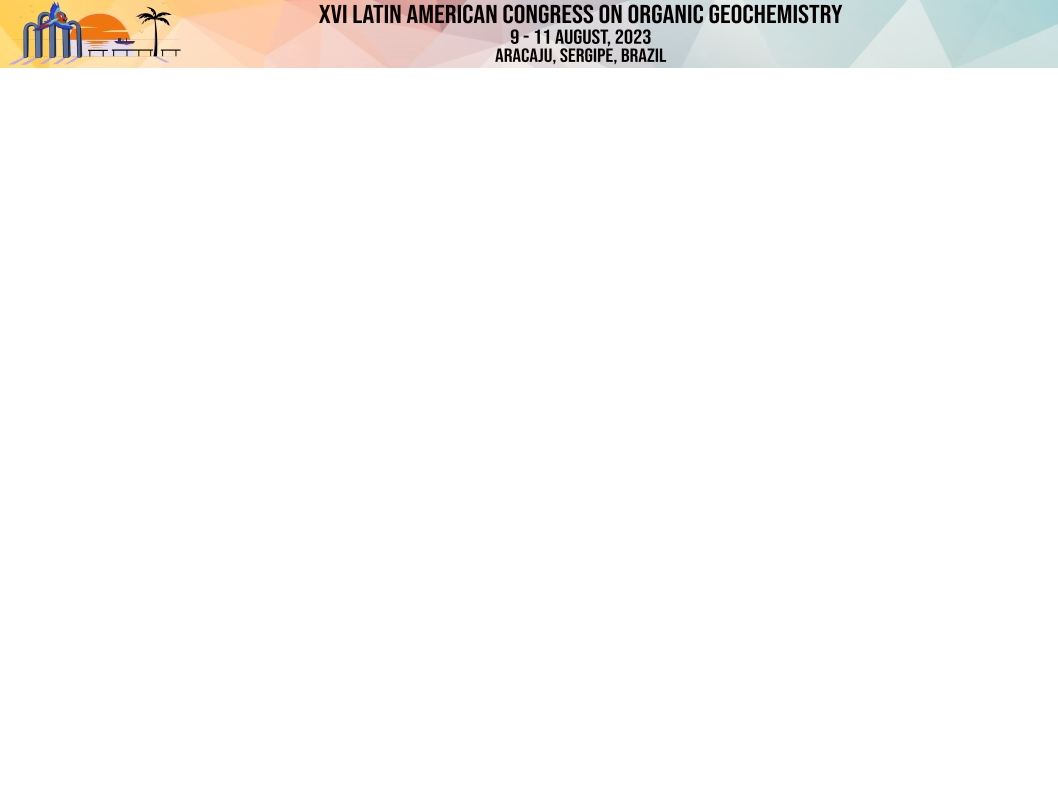
\includegraphics[width=\paperwidth,
height=\paperheight]{images/fundo.jpg}
}

{ \begin{frame}
\begin{flushright}
\frametitle{Objectives}
\end{flushright}


\begin{flushright}
    \begin{columns}
    \column{0.4\textwidth}
        \centering
        
    \column{0.6\textwidth}
        \centering
	      
    \end{columns}

\end{flushright}


\end{frame} }



% INTRODUÇÃO
\section{Introduction}
% METODOLOGIA
\section{Methodology}
% RESULTADOS E DISCUSSÕES
\section{Results and Discussion}
% CONCLUSÕES 
\section{Conclusion}






%%%%%%%%% FINAL %%%%%%%%%%%%%%
\usebackgroundtemplate{
\centering

\includegraphics[width=\paperwidth,height=\paperheight]{images/base.png}
}
\begin{frame}[allowframebreaks]
\frametitle{References}
%\beamertemplatetextbibitems
\tiny
\bibliographystyle{apalike}
\bibliography{references}
\end{frame}
}
\makeatother

{
\usebackgroundtemplate{
\centering

\includegraphics[width=\paperwidth,height=\paperheight]{images/agradecimento.png}
}	
\begin{frame}
\end{frame}
}


\end{document}
